\section{Experimental setup}\label{header-n31}

The aim of this project is to evaluate the performances of deep networks
in an image multi-classification task. More in detail, it consists into
map fruit and vegetables images on ten classes: \emph{apple},
\emph{banana}, \emph{plum}, \emph{pepper}, \emph{cherry}, \emph{grape},
\emph{tomato}, \emph{potato}, \emph{pear}, and \emph{peach}.

\subsection{Dataset}\label{header-n33}

The dataset consists of a wide series of images that depict different
types of fruit and vegetables. It is downloadable by following this
\href{https://www.kaggle.com/moltean/fruits}{link}. The original dataset
is already divided into training and test set. For each set, each type
of fruit and vegetables is divided according to its main characteristics.
For instance, the fruit type "apple" can be divided into a lot of
sub-categories according to its variety (apple Golden, apple Granny
Smith, apple Pink Lady, etc) and its color (yellow, red, green, etc). In
the dataset, for each type-feature pair, there is a folder that contains
the related pictures. The dataset is not used as is but it is modified
and reorganized to perform the assigned task. First of all, the split
between training and test set is removed in order to compose a single
set of images. Secondly, the sub-types of fruit and vegetables are
grouped together. This means that all apple sub-types belonging to the
same class. Finally, only the 10 requested types of fruit and vegetables
are considered (apple, banana, plum, pepper, cherry, grape, tomato,
potato, pear, and peach), while the others are removed. Now the dataset is
composed of ten folders that contain the images relating to the ten
classes. The figure below shows an example picture for each class.

\begin{figure}[h!]
\centering
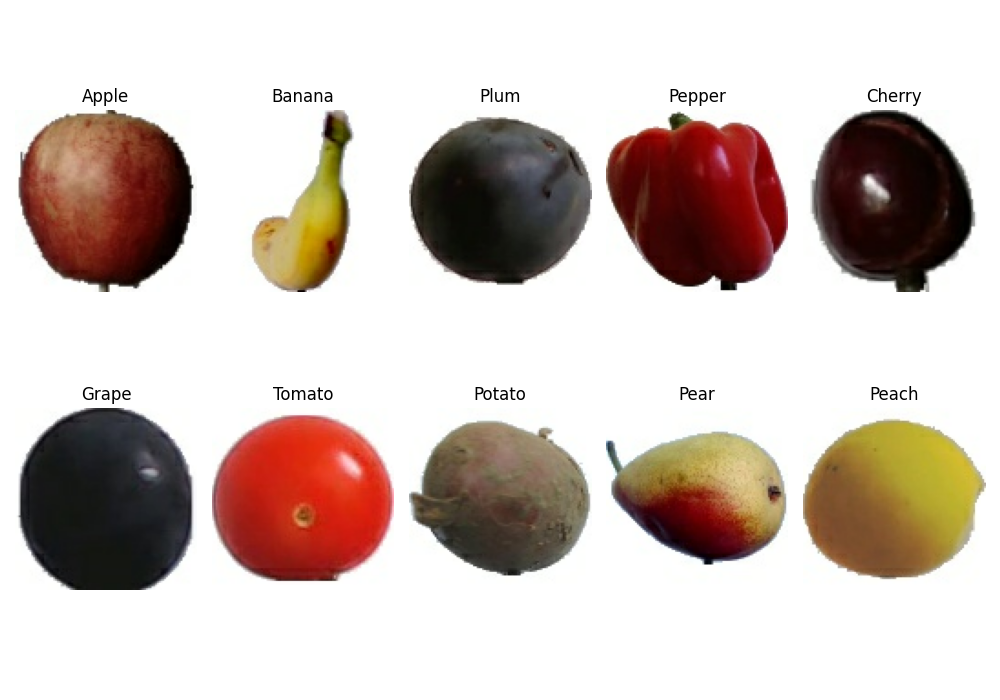
\includegraphics[width=0.9\linewidth]{../images/fruit-categories.png}
\caption{The classes of picture that models have to predict}
\end{figure}

To better understand how the dataset is composed, the following table
and graphic show the number of samples for each class and the total
amount of pictures

\begin{longtable}[]{@{}ll@{}}
\toprule
\textbf{Class} & \textbf{N. of samples}\tabularnewline
\midrule
\endhead
Apple & 8538\tabularnewline
Banana & 1258\tabularnewline
Cherry & 4592\tabularnewline
Grape & 4565\tabularnewline
Peach & 1640\tabularnewline
Pear & 6070\tabularnewline
Pepper & 3304\tabularnewline
Plum & 1766\tabularnewline
Potato & 2404\tabularnewline
Peach & 6810\tabularnewline
\textbf{Total} & \textbf{40947}\tabularnewline
\bottomrule
\caption{The amount of samples for each class}
\end{longtable}

\begin{figure}[h!]
\centering
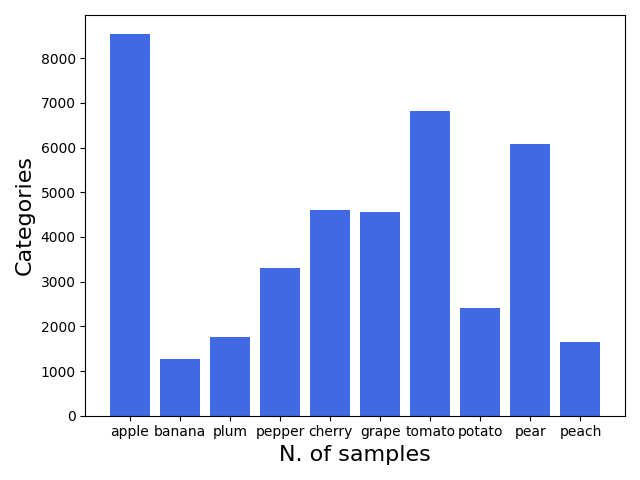
\includegraphics[width=0.9\linewidth]{../images/n_samples.png}
\caption{The amount of samples for each class}
\end{figure}

\subsection{Data preprocessing}\label{header-n75}

The problem's data (the images) have to be properly elaborated before
being used by models. The data preprocessing phase aims to make the
dataset easier to analyze, in order to increase the models' performance and to
reduce the training time. The preprocessing pipeline, applied for each
picture, is composed of two steps:

\begin{itemize}
\item
  \textbf{scaling:} the image is resized form 100x100 pixels to 32x32
  pixels using the bilinear interpolation algorithm
\item
  \textbf{normalization:} the pixels RGB channel values, originally in
  the {[}0, 255{]} range, are standardized to be in the {[}0, 1{]}
  range.
\end{itemize}

\subsection{Experiments evaluation}\label{header-n82}

After the preprocessing pipeline, the data are ready to be used by the
learning machines. Cross-validation is used to evaluate the models'
performances, in particular the Hold-out technique. This method consists
into split the dataset in two separate sets: the training set (used to
train the learning algorithms) and the test set (used to evaluate the
models' performance). In this case, the split is 80\% and 20\% for
training and test set respectively. The union between them form an holdout. The
experiments are executed over 20 different holdouts. The
\href{https://scikit-learn.org/stable/modules/generated/sklearn.model_selection.StratifiedShuffleSplit.html}{method}
used to compute the holdouts is implemented in the sklearn library. This
method randomly splits the original dataset preserving
the percentage of samples for each class. In the project code, it is set with 42 as a random
state parameter. To numerically evaluate the models the following
metrics are used:

\begin{itemize}
\item
  \textbf{loss function value}: the value of the models' loss function
\item
  \textbf{accuracy:} the ration between the correct predictions and the
  total number of samples.
\end{itemize}

The final results are the mean and the standard deviation of the metrics
obtained by the learning machines using each holdouts (both for training
and validation phases). These results and the related conclusions are
finally validated using the Wilcoxon Signed-Rank test with a p-value
threshold of 0.01. It is a non-parametric statistical test to compare
hypotheses made on repeated measures. In addiction, for each model, the
trend of the metrics during the training phase are plotted to understand
how the model learns during the epochs succession. Metrics history is tracked only for the first holdout.